\chapter{Preliminaries}

%-------------------------------------------------------------
%Here goes the introduction of transport between quantum dots. stil need to add important considerations like the smooth varying DOS. Not so discrete. 
%Assumption: 
%   1-Only the level immediately at the bottom of the fermi       level is considered
\section{Transport in Quantum Dots (QDs)}
Quantum mechanical effects are visible when the system size is of the order of the de Broglie wavelength \citep[(1.1)]{bimberg_quantum_1999}
\[
\lambda_{f}=\frac{h}{\sqrt{3m_{\mathsf{eff}}k_{B}T}}
\]
 where $m_{\mathsf{eff}}$ is the electron effective mass in the crystal.
Since $m_{\mathsf{eff}}$ can be much smaller than the free electron mass in some semiconducting materials, size quantization effects can be observed at system of sizes $\sim100\mbox{nm}$ \citep[2.1]{sindel_numerical_2005}. A device confined in the three dimensions up to this length-scale will present the behavior of a $0$D quantum system, which is what we call a Quantum Dot (QD).\\

Nowadays, QDs can be manufactured with several methods, forms and orientations \citep{bimberg_quantum_1999}. According to their orientation with respect to the based 2D-plane , two main types of QDs can be distinguished : Vertical (Figure \ref{QD-figuresA}) and lateral (Figure \ref{QD-figuresB}) QDs. Both types of of quantum dots have $3$-main gates. Two of them are the Drain $V_D$ and source $V_S$ gate voltages used to control the current trough the QD. The third one is the gate voltage $V_G$. This one controls the electron confinement inside the QD. Therefore, tuning the gate voltage it is possible to control accurately the energy levels of the QD. 



\begin{figure}[hbt]
\centering
\subfloat[\label{QD-figuresA}\label{QD-figures}]{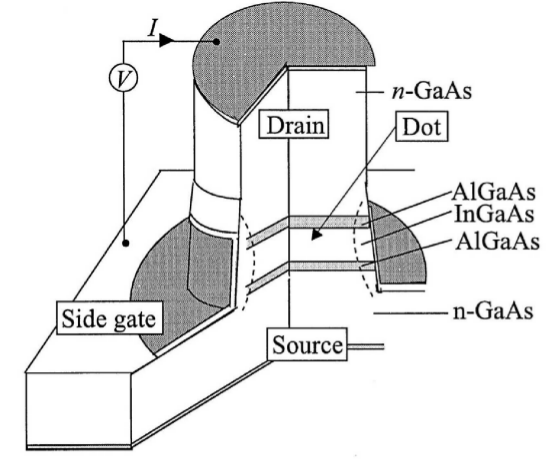
\includegraphics[scale=0.3]{IMAGES/Preliminars/VerticalQD.png}}\hspace{6mm}
\subfloat[\label{QD-figuresB}]{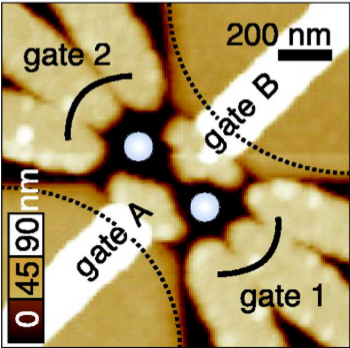
\includegraphics[scale=0.4]{IMAGES/Preliminars/QD-horizontal.png}}

\caption{ a) Vertical quantum dot.  b)Atomic force microscopy
picture of two coupled lateral QDs (bright central circles). Gates 1 and 2 act as drain and source voltage. A negative
voltage is applied at gates $A$,$B$ to allow the formation of the droplets inside the free space in the 2D electron gas. \Source{\cite{holleitner_probing_2002}} }

\end{figure}


Ideally, the energy spectrum of a QD is a discrete set of energy levels resembling the spectrum of an atom. However, when the QD is connected to metallic leads these energy levels hybridized with respect to a hybridization parameter $\Gamma$ which depends on the voltage connecting the lead with the dots $V_L$.
\begin{equation}
    \Gamma = \pi \Vert V_l \Vert^2 
\end{equation}



The great advantage of QDs is that their spectrum looks pretty similar
to the spectrum of an atom, which is a discrete set of energy levels.
% Indeed we can model an ideal single-electron QD as a quantum well
% with a negative constant potential inside the dot . For example an
% spherical quantum dot with radius $R$ will take the following Schr�dinger
% Hamiltonian 

% \[
% H\Psi(r)=\left(\frac{\hbar^{2}}{2m^{*}}\nabla^{2}+V(r)\right)\Psi(r)\ ,\ \textrm{with }V(r)=\begin{cases}
% -V_{0} & r<R\\
% 0 & r\geq R
% \end{cases}.
% \]


% The 
% the energy level spacing is  \citep[Equation (5.44)]{bimberg_quantum_1999}

% \[
% \delta E\propto\frac{1}{R^{2}}.
% \]

On an ideal QD the energy

%------------------------------------------------------------
\subsection{The Anderson Model}

For more electrons, the coulomb
repulsion inside the dot is important.. Hence, using the Hunds rule we know that the energy levels should be filled from lower to higher energies with two electrons with different spin at each state. Taking in account
all these interactions we can get to a second quantization QD-Hamiltonian
of the form \citep[(3.2)]{sindel_numerical_2005}

\[
H_{d}=\sum_{i\sigma}\epsilon_{di}d_{i\sigma}^{\dagger}d_{i\sigma}+\sum_{i}U_{i}\hat{n}_{i\uparrow}\hat{n}_{i\downarrow}+\sum_{\sigma\sigma',i\neq j}U_{ij}\hat{n}_{i\sigma}\hat{n}_{j\sigma'}-\mu_{B}gB\sum_{i}S_{i}^{z}+J\sum_{i\neq j}\mathbf{S}_{i}\cdot\mathbf{S}_{j}.
\]


Where $\sigma\in\{\uparrow,\downarrow\}$, $d_{i\sigma}^{\dagger}\left(d_{i\sigma}\right)$
is the dot creation(annihilation) operator,$\hat{n}_{i\sigma}:=d_{i\sigma}^{\dagger}d_{i\sigma}$
is the particle number, $\mathbf{S}_{i}$ is the spin-vector, $\epsilon_{di}$
is the energy of the $i^{\mbox{th}}$-level in the dot, $U_{i}$ is
the coulomb repulsion between electrons in the same energy level $i$,
$U_{ij}$ is the coulomb interaction between electrons in different
levels (And therefore smaller than $U_{i}$), \textbf{$B$} is an
applied magnetic field in the $\hat{z}$-direction and $J$ is the
term representing the Zeeman splitting. We now use that we can control
the energy levels of the QD by switching set the gate-voltage, such
that we only take in consideration one level in the QD. Taking this
assumption the dot Hamiltonian becomes \\

\begin{figure}[h]
\centering
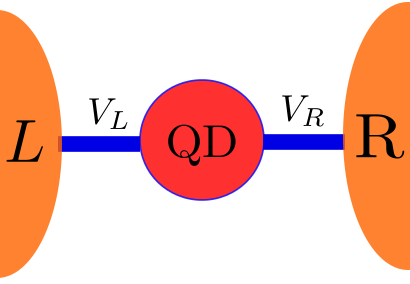
\includegraphics[scale=0.45]{IMAGES/QD_transport.png}\caption{\label{QD-transport}Transport measurement scheme in the QD. }
\end{figure}


\[
H_{d}=\sum_{\sigma}\epsilon_{d}d_{\sigma}^{\dagger}d_{\sigma}+U\hat{n}_{\uparrow}\hat{n}_{\downarrow}-\mu_{B}gBS^{z}.
\]


Since we are interested in implementing transport measurements through
the QD we need to link the dot to two metallic leads ($L$(left) and
$R$(right)) so that electron conduction can be performed (\ref{QD-transport}).
For this we can add two new hamiltonians in second quantization that
represent the energy of the electrons inside the leads $H_{lead}$
and the interaction between the leads and the quantum dot $H_{int}$.
These hamiltonians take the form 

\begin{eqnarray*}
H_{lead} & = & \sum_{\mathbf{k}\sigma l}\epsilon_{\mathbf{k}l}c_{\mathbf{k}\sigma l}^{\dagger}c_{\mathbf{k}\sigma l}\\
H_{int} & = & \sum_{\mathbf{k}\sigma l}V_{\mathbf{k}l}c_{\mathbf{k}\sigma l}^{\dagger}d_{\sigma}+V_{\mathbf{k}l}^{*}d_{\sigma}^{\dagger}c_{\mathbf{k}\sigma l},
\end{eqnarray*}


where $\mathbf{k}$ represents the possible crystal momentums in the
leads, $l\in\{L,R\}$, $c_{\mathbf{k}\sigma l}^{\dagger}(c_{\mathbf{k}\sigma l})$
creates(annihilates) an electron with momentum $\mathbf{k}$ and spin
$\sigma$ in the lead $l$, $\epsilon_{\mathbf{k}l}$ is the energy
of the electron in the leads and $V_{\mathbf{k}l}$ is a hopping exchange
term between the leads and the QD. Therefore the final form of the
transport Hamiltonian through the quantum dot takes the form of 
\begin{eqnarray}
H & = & H_{d}+H_{lead}+H_{int}\nonumber \\
 & = & \sum_{\sigma}\epsilon_{d}d_{\sigma}^{\dagger}d_{\sigma}+U\hat{n}_{\uparrow}\hat{n}_{\downarrow}-\mu_{B}gBS^{z}+\sum_{\mathbf{k}\sigma l}\epsilon_{\mathbf{k}l}c_{\mathbf{k}\sigma l}^{\dagger}c_{\mathbf{k}\sigma l}+\sum_{\mathbf{k}\sigma l}V_{\mathbf{k}l}c_{k\sigma l}^{\dagger}d_{\sigma}+V_{\mathbf{k}l}^{*}d_{\sigma}^{\dagger}c_{\mathbf{k}\sigma l}.\label{eq:Anderson}
\end{eqnarray}


This hamiiltonian is a particular case of a more general theory for
impurities in metals known as the Anderson model \citep{anderson_localized_1961}.


%------------------------------------------------------------
\section{Kondo Effect}

In the early 30s the physicist where intrigued by the observation of a resistance minimum in some metals at low temperatures $(\sim 10K)$ \cite{sindel_numerical_2005} . The phenomenon received the name of Kondo effect \citep{hewson_kondo_1997}. This effect is attributed to the electron-scattering with the magnetic impurities present in the materials. 

Using perturbation theory is possible to explain how this spin flip produces a  temperature dependent effect which  introduces an additional logarithmic term to the resistivity of the form

\begin{equation}
\rho_{Kondo}(T) \propto \ln{\left( \frac{T_{kondo}}{T} \right)},
\label{logKondo}
\end{equation}



which occurs due to the spin-flip between the particles in the impurity and in the reservoir. The entire resistivity including  and 

We can seen that under the scale of temperature defined by $T_k$ the Kondo effect dominates over all other interactions. However, there is a fundamental problem in the Kondo model. For temperatures much smaller than $T_K$ the resistivity diverges. This problem is solved by applying a re-normalization group approach to treat the strong correlations appearing at low temperatures. In the Kondo problem a logarithmic discretization is used. The numerical procedure receives the name of Numerical renormalization Group (NRG). 


\subsection{Kondo Effect in QDs}


The problem of magnetic impurities in metals can be treated using the Anderson model in a similar form as the transport
 in quantum dots. Hence, it is not a surprise that Kondo Effect could also occur in QDs. When an odd number of electrons is in the QD the last level bellow the Fermi energy is half-occupied and hence the dot is magnetized. The unlocalized electrons in the reservoirs then interact with this localized electron . Spin-flip can occur as in the case of  magnetic impurities in metals. At low temperatures, this magnetic  interaction gives rise to strong quantum correlations that favor the formation of a singlet state between the localized electron and the electrons in the leads. As a result, the zero-bias density of states is increased producing a zero-bias conductance peak. \\

Note that the physical implications of the Kondo effect  between the case of magnetic impurities in metals and transport through QD are different. The reason for this is difference in the dimension in both processes . While the scattering at 3D systems against magnetic impurities should produce a drop in the conductivity at low temperatures, the scattering in 0D systems enhances the conductivity of the QD due to the few scattering directions. This implies that the Kondo Effect in QDs acts in the opposite way as in the impurity case. 
















% The next part of thess preliminaries will be to compute the conductivity
% through the QD as a function of the gate voltage.
% In regular metals the Kondo effect manifests as a drop in conductivity
% under a certain Kondo temperature $(T_{Kondo})$ due to spin- scattering
% between the conduction electrons and the impurities of the material.
% The Anderson models, hence the NRG, are the perfect tools to study
% the physics of impurieties. Thus the computations we previously developed
% in this chapter will provide the right formalism to introduce the
% Kondo physics. This study will be an important part of the prelimiraries
% in the final document. 



%-----------------------------------------------------------

